\PassOptionsToPackage{warn}{textcomp}

\documentclass[12pt,a4paper]{article}
\usepackage{amsmath, amssymb}
%\usepackage[warn]{mathtext}
\usepackage[T2A]{fontenc}
\usepackage[utf8]{inputenc} 
\usepackage[russian]{babel} 

\usepackage{textcomp}
%\DeclareSymbolFont{T2Aletters}{T2A}{cmr}{m}{rm}
\usepackage{epstopdf}
\usepackage[lastpage,user]{zref}
\usepackage{geometry, graphics, graphicx}

\geometry
{
	a4paper,
	total={210mm,297mm},
	left=20mm,
	right=20mm,
	top=25mm,
	bottom=20mm,
}

\usepackage{hyperref}

\hypersetup{
	    bookmarks=true,         % show bookmarks bar?
	%    unicode=false,          % non-Latin characters in Acrobat’s bookmarks
	%    pdftoolbar=true,        % show Acrobat’s toolbar?
	%    pdfmenubar=true,        % show Acrobat’s menu?
	%    pdffitwindow=false,     % window fit to page when opened
	%    pdfstartview={FitH},    % fits the width of the page to the window
	%    pdftitle={My title},    % title
	%    pdfauthor={Author},     % author
	%    pdfsubject={Subject},   % subject of the document
	%    pdfcreator={Creator},   % creator of the document
	%    pdfproducer={Producer}, % producer of the document
	%    pdfkeywords={keyword1, key2, key3}, % list of keywords
	%    pdfnewwindow=true,      % links in new PDF window
		colorlinks=true,       % false: boxed links; true: colored links
		linkcolor=blue!80!black,          % color of internal links (change box color with linkbordercolor)
		citecolor=green!30!black,        % color of links to bibliography
		filecolor=magenta!801black,      % color of file links
		urlcolor=blue!50!black           % color of external links
}

\usepackage{color}
\usepackage[usenames,table]{xcolor}

\colorlet{linkequation}{red!80!black}

\newcommand*{\SavedEqref}{}
\let\SavedEqref\eqref
\renewcommand*{\eqref}[1]{%
	\begingroup
	\hypersetup{
		linkcolor=linkequation,
		linkbordercolor=linkequation,
	}%
	\SavedEqref{#1}%
	\endgroup
}



% ----------------------------------------
% ------------Колонтитулы-----------------
\usepackage{fancyhdr}
\pagestyle{fancy}

\fancyhead{}
\rhead{\textbf{Выпонила:\\} \emph{Кузина Мария}}
\chead{\textsf{СПбПУ}\\им. Петра Великого}
\lhead{\textbf{Практическое задание №1\\} \emph{вариант 12}}
\lfoot{\scriptsize
	\textbf{UPD.:}~\emph{\today}\quad	
}
\cfoot{}
\rfoot{\thepage /\zpageref{LastPage}}

%% Листинги
%\definecolor{MatlabCellColour}{RGB}{252,251,220}
%\definecolor{mygreen}{RGB}{28,172,0} % color values Red, Green, Blue
%\definecolor{mylilas}{RGB}{170,55,241}
%\usepackage{listings}

\usepackage[framed,numbered,autolinebreaks,useliterate]{mcode}


%% Операторы
\usepackage{amsmath, amsopn}
\DeclareMathOperator{\sigm}{sigm}

\usepackage{hyperref}
\usepackage{diffcoeff}
\usepackage[final]{showlabels}

\usepackage{upgreek}
\newcommand{\del}{\Updelta}

\usepackage[labelsep=period]{caption}
\usepackage{float}

\newcommand{\ffnn}{\texttt{FFNN}}
\newcommand{\ff}{\texttt{FF}}
\newcommand{\ns}{\texttt{Ns}}

%\renewcommand{\thesection}{\Asbuk{section}}
\renewcommand{\appendixname}{Приложение}

\usepackage{diffcoeff}
%\usepackage{enumitem}
%\renewcommand{\labelitemii}{\textopenbullet}

\renewcommand{\v}{\mathbf}

\usepackage{pgfplots}
\usetikzlibrary{calc}
\usetikzlibrary{graphs,graphs.standard}
\tikzgraphsset{declare={polygon_n}{[clique]\foreach\x in\tikzgraphV{\x/}}}
\usetikzlibrary{shapes.geometric}


\begin{document}
\section*{\Large\center Реализация нейронной сети FFNN
для анализа и классификации геометрических фигур}    
\section*{Условие}
\noindent
Написать программу моделирования нейронных сетей (НС) 
заданного типа и показать их работоспособность на практических примерах использования НС для указанной задачи.
Параметры НС представлены в таблице \ref{tbl:01}.

\begin{table}[h]
	\center
	\caption{Параметры модели \label{tbl:01}}
\begin{tabular}{lc|l}
\textbf{Вход} & & Изображения на некотором фоне одной из 5 геометрических фигур \\
\textbf{Выход} & & Какая фигура \\
\textbf{Тип НС} & & \ffnn \\
\textsf{\ns} &  & Число элементов в скрытом слое
\end{tabular}
\end{table}

\section{Постановка задачи, связанной с практическим \newline применением НС}
Компьютерное зрение на основе методов распознавания геометрической 
формы получило широкое распространие на производстве в таких областях 
как промышленный осмотр, идентификация, и автоматический контроль
качества продукции. 
В задаче автоматической сборки, значительный объем информации о детали
необходимо распознавать и классифицировать, а ее ориентация должна быть 
автоматически определена, прежде чем робот (манипулятор) сможет ухватиться 
за изделие или его часть. 
Также применяются методы распознавания формы
для оптического распознавания символов, рукописного текста,
а также медицинских изображений, и.т.д. \cite{hou1999}.\\[6pt]
\noindent
\emph{Базовой задачей}, предваряющей перечисленные выше, является
задача распознавания и классификации плоских геометрических фигур
таких как треугольник, квадрат, пятиугольник, шестиугольник и круг 
(многоугольник с количеством сторон $\sim100$).

\section{Описание теоретической базы рассматриваемой \newline модели НС}
Нейронные сети прямого распространения (feed forward neural networks, 
\ff\,или \ffnn) передают информацию от входа к выходу \cite{Rosenblatt1958}. 
Сети \ffnn, описываются в виде набора слоёв клеток (нейронов). Причём, существуют входные, скрытые и выходные слои
(рис. \,\ref{fig:01})
Нейроны одного слоя не связаны между собой, а соседние слои обычно 
связаны полностью (каждый с каждым). В данной работе будем рассматривать только полносвязные \ffnn.

\begin{figure}[tbh!]
	\centering
	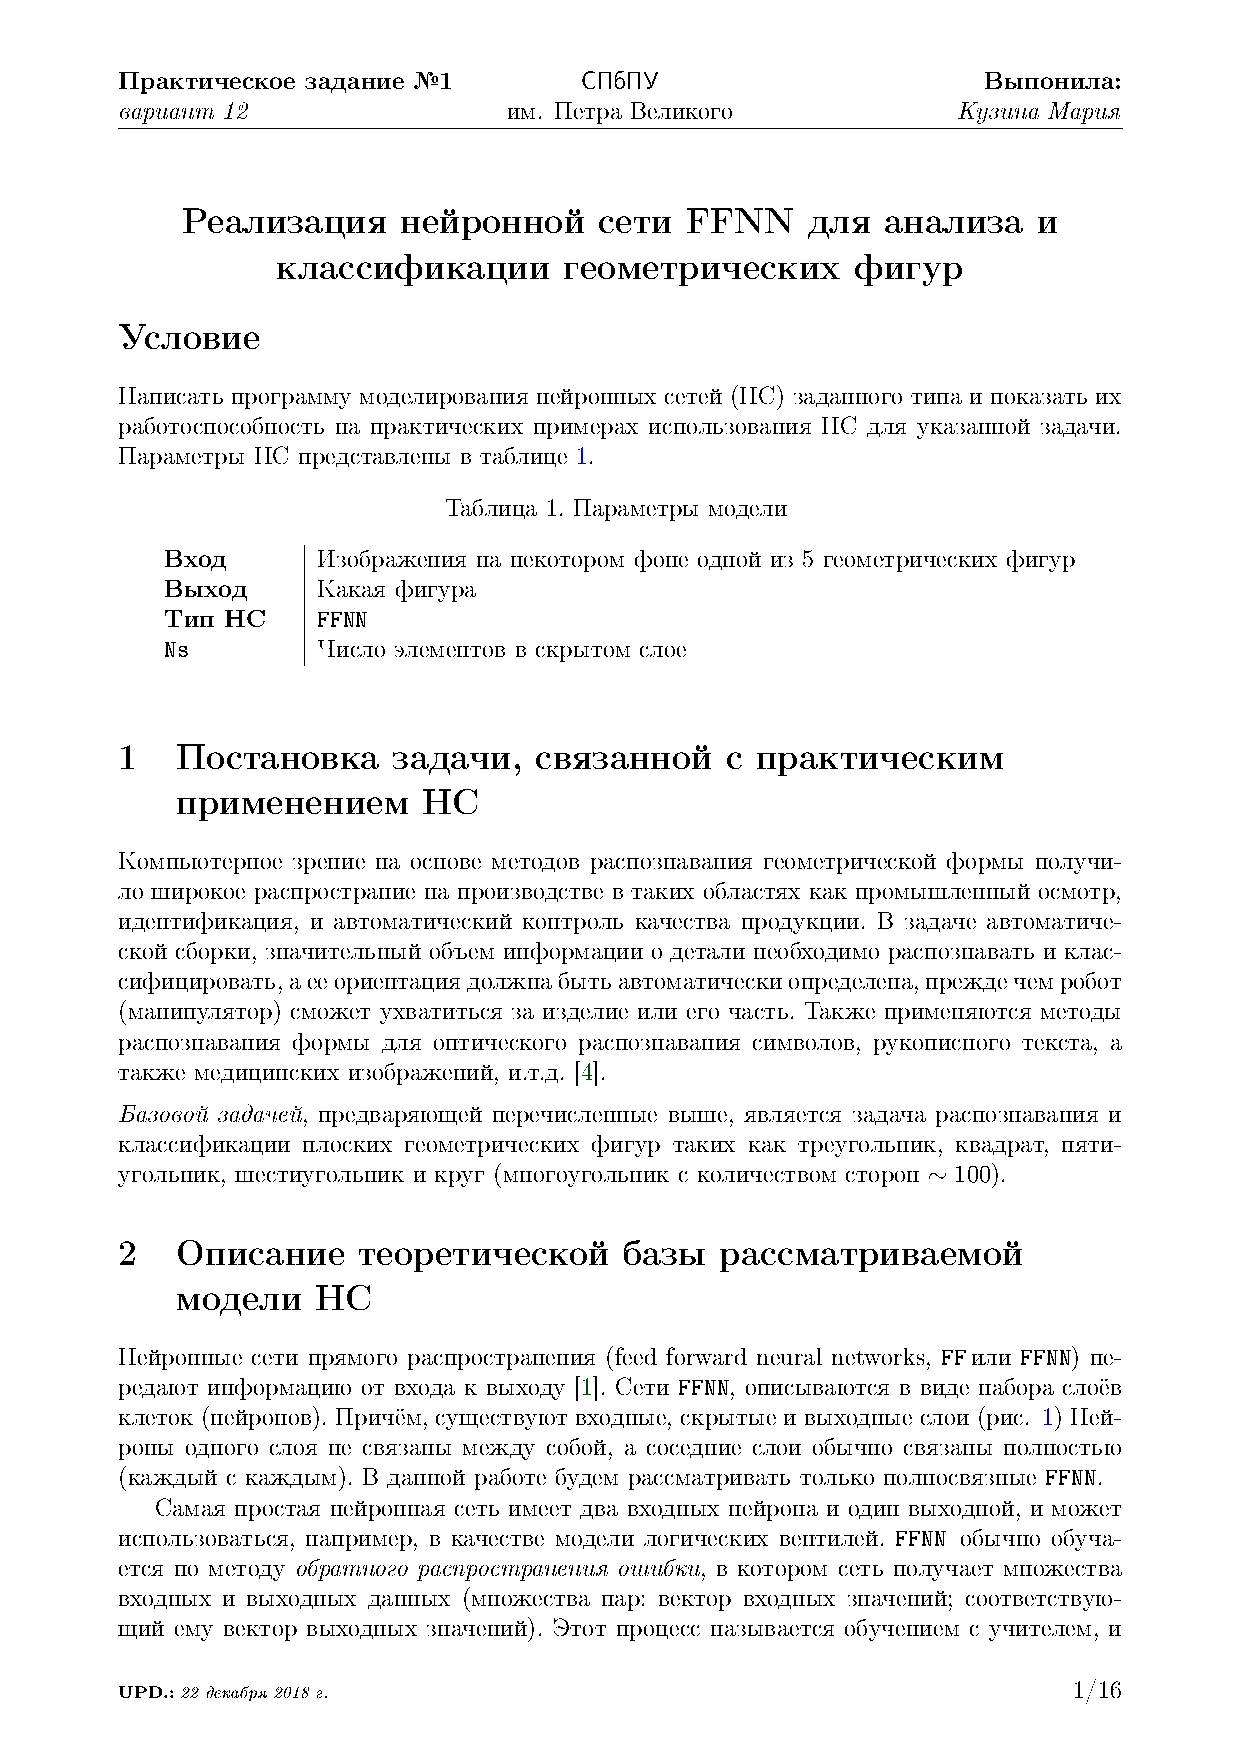
\includegraphics[width=0.3\textheight]{_ref_/ffnn}
	\caption{НС прямого распространения\label{fig:01} \cite{NNzoo}}
\end{figure}

Самая простая нейронная сеть имеет два входных нейрона и один выходной, и может использоваться, например, в качестве модели 
логических вентилей. \ffnn\, обычно обучается по методу \emph{обратного распространения ошибки}, в котором сеть получает множества входных и выходных данных (множества пар: {вектор входных значений; соответствующий ему вектор выходных значений}). Этот процесс называется обучением с учителем, и он отличается от обучения без учителя тем, что во втором случае множество выходных данных сеть составляет самостоятельно. 

Упомянутая выше \emph{ошибка} является разницей между вводом и выводом. Если у сети есть достаточное количество скрытых нейронов, она теоретически способна смоделировать взаимодействие между входным и выходными данными. 

На практике такие сети используются редко, но их часто комбинируют с другими типами для получения новых.\\[12pt]
\noindent
Рассмотрим вычисления в рамках одного нейрона \ffnn.

\subsubsection*{Активация нейрона и вычисление выхода}
%\begin{figure}[tbh!]
%%	\centering
%	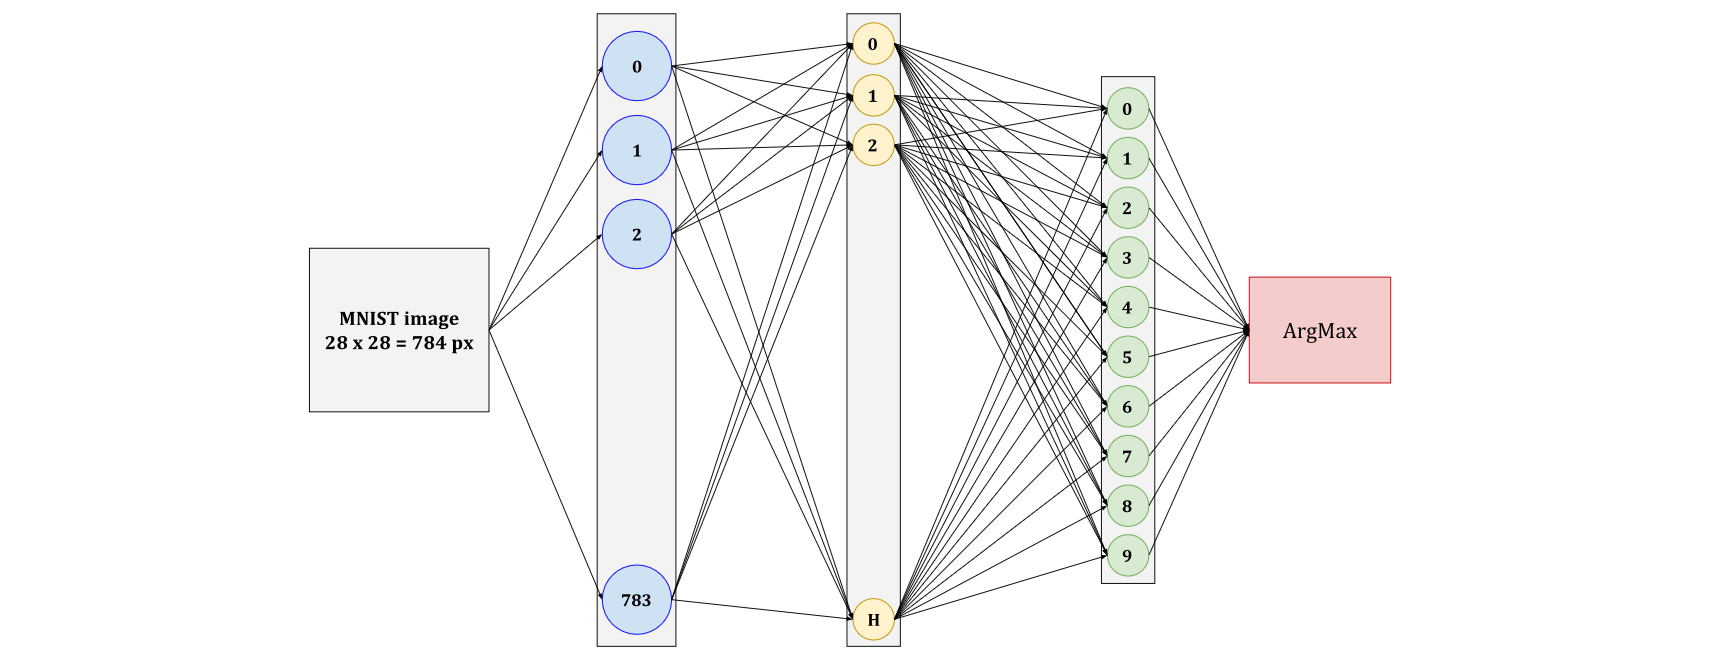
\includegraphics[]{_ref_/mnist_nn_single_hide}
%	\caption{НС прямого распространения\label{fig:01} \cite{NNzoo}}
%\end{figure}
Активация нейрона происходит по правилу \eqref{eq:01}
в векторном виде 
\begin{equation}\label{eq:01}
a(x) = b + \v{w}^T\v{x}.
\end{equation}
Здесь $\v{x}$ --- входной вектор,
$\v{w}$ --- вектор весовых коэффициентов, $b$ --- отклонение (bias).

Активационные функции $g(x)$ бывают разных видов. 
Наиболее распрострненными являются 
\emph{сигмоида}, приведена на рис.\,\ref{fig:02},
\begin{equation}\label{eq:04}
g(x) = \mathrm{sigm}{\,x} = \dfrac{1}{1+\exp{(-x)}},
\end{equation}
и \emph{гиперболический тангенс}, на рис.\,\ref{fig:03}
\begin{equation}\label{eq:05}
g(x) = \tanh{x} = \dfrac{\exp(2x)-1}{\exp{(2x)}+1}.
\end{equation}
В качестве активационной функции также используется функция \eqref{eq:02} вида
\begin{equation}\label{eq:02}
g(x) = 
\begin{cases}
1,~\v{w}^T\v{x}>\varepsilon,\\
0,~\v{w}^T\v{x}\geqslant\varepsilon,
\end{cases}
\end{equation}
где $\varepsilon$ --- пороговое значение (\texttt{treshold}).\\

Результат (конечный выход нейрона) $h(x)$ вычислятся \eqref{eq:03} подстановкой 
\begin{equation}\label{eq:03}
h(x) = g(a(x)) = g(b + \v{w}^T\v{x}).
\end{equation}

\begin{figure}[tbh!]
\begin{minipage}[b]{0.45\linewidth}
	\centering
	\begin{tikzpicture}
	\begin{axis}[
	xmin=-14.5, xmax=14.5,
	ymin=-1.5, ymax=1.5,
	axis lines=center,
	axis on top=true,
	domain=-14.5:14.5,
	ylabel=$y$,
	xlabel=$x$,
	]
	
	\addplot [mark=none,draw=red!50!black,ultra thick,samples=100] {1/(1+exp(-\x))};
	\node [left, red!50!black] at (axis cs:-1,0.7) {$y = \sigm{x}$};
	
	%% Add the asymptotes
	\draw [blue, dotted, thick] (axis cs:-2.5,-1)-- (axis cs:0,-1);
	\draw [blue, dotted, thick] (axis cs:+2.5,+1)-- (axis cs:0,+1);
	\end{axis}
	\end{tikzpicture}
\caption{Сигмоида}
\label{fig:02}
\end{minipage}
\hspace{0.5cm}
\begin{minipage}[b]{0.45\linewidth}
	\centering
	\begin{tikzpicture}
	\begin{axis}[
	xmin=-14.5, xmax=14.5,
	ymin=-1.5, ymax=1.5,
	axis lines=center,
	axis on top=true,
	domain=-14.5:14.5,
	ylabel=$y$,
	xlabel=$x$,
	]
	
	\addplot [mark=none,draw=red!50!black,ultra thick,samples=100] {tanh(\x)};
	\node [left, red!50!black] at (axis cs: -1,0.7) {$y = \tanh{x}$};
	
	%% Add the asymptotes
	\draw [blue, dotted, thick] (axis cs:-2.5,-1)-- (axis cs:0,-1);
	\draw [blue, dotted, thick] (axis cs:+2.5,+1)-- (axis cs:0,+1);
	\end{axis}
	\end{tikzpicture}
	\caption{Гиперболический тангенс}
	\label{fig:03}
\end{minipage}
\end{figure}



\section{Описание разработанных ПМ и решение задачи}
%Решение задачи с использованием НС и оценка качества решения, план экспериментов по проверке работоспособности, результаты моделирования
%(в табличной и графической форме).

Для решения поставленной задачи распознавания геометрических фигур на фоне различных цветов с помощью \ffnn\,нейронной сети
реализуем обучающую и тестовую выборки изображений. В качестве геометрических фигур рассмотрим правильные $n$--угольники. 
Для $n=3$ --- треугольник,
$n=4$ --- квадрат, $n=5$ --- пятиугольник, $n=6$ --- шестиугольник и $n=100$ --- круг (представлены на рис.\,\ref{fig:04}).

\begin{figure}[tbh!]
	\center
	\newdimen\R
	\R=.6cm
	\begin{tikzpicture}
	% Indicate the boundary of the regular polygons
	\draw[fill=red!25] (0:\R) \foreach \x in {120,240} {
		-- (\x:\R)
	} -- cycle (90:\R);
	\draw[fill=green!25,xshift=2.5\R] (0:\R) \foreach \x in {90,180,...,359} {
		-- (\x:\R)
	} -- cycle (90:\R);
	\draw[fill=blue!25,xshift=5.0\R] (0:\R) \foreach \x in {72,144,...,359} {
		-- (\x:\R)
	} -- cycle (90:\R);
	\draw[fill=magenta!25,xshift=7.5\R] (0:\R) \foreach \x in {60,120,...,359} {
		-- (\x:\R)
	}-- cycle (90:\R);
	\draw[fill=black!25,xshift=10.0\R] (0:\R) \foreach \x in {3.6,7.2,...,359} {
		-- (\x:\R)
	} -- cycle (90:\R);
	\end{tikzpicture}
	\caption{n-угольники}
	\label{fig:04}
\end{figure}



Был реализован алгоритм, позволяющий получить изображения указанных геометрических фигур различных размеров и цветов. Предусмотрена возможность поворота фигуры на некоторый случайный угол.

\subsubsection*{Файлы \texttt{Matlab}:}
\verb|gen_set_of_ngons.m|\\
\verb|gen_ngon_image.m|\\
\verb|run_gen_ngon.m|\\[6pt]

После того, как изображения были сгенерироны и сохранены на жестком диске, скомпануем по ним сами выборки.
%Файл \texttt{Matlab}:\\
%\verb|load_dataset.m|

\subsubsection*{Выборка \textnumero\,1 ''Сложная''}
Всего 70 тысяч примеров -- изображений размером $28\times28$ пикселей, 
по 14 тысяч на каждую фигуру. При этом 60 тысяч отнесем к обучающей выборке, а оставшиеся 10 -- к тестовой (валидационной).

Фигуры расположены произвольно относительно центра изображения, произведён поворот на случайный угол. Цвет фигуры и цвет фона также случайные, см. рис.\,\ref{fig:05}.

\begin{figure}[H]
	\centering
	\includegraphics[scale=0.125]{_ref_/3-gone-smpl}	
	\includegraphics[scale=0.125]{_ref_/4-gone-smpl}
	\includegraphics[scale=0.430]{_ref_/5-gone-smpl}	
	\includegraphics[scale=0.125]{_ref_/6-gone-smpl}	
	\includegraphics[scale=0.125]{_ref_/100-gone-smpl}						
	\caption{Примеры сгенерированных фигур}
	\label{fig:05}
\end{figure}



Все цветные изображения переведём в оттенки серого и преобразуем в одномерный массив длиной 784 элемента. Размер выборки такой же, как и в задаче распознавания \ffnn, -- сетью рукописных цифр MNIST. В типовом решении последней задачи используются следующие параметры персептрона:
\begin{itemize} 
\item число входов нейронной сети: 784 (= $28\times28$);
\item число нейронов в скрытом слое: 100;
\item число выходных нейронов: 10 (по одному на каждую цифру) с выходным значением от 0 до 1.
\end{itemize}
Такая сеть тренируется на парах ($I_{j},\,v_{j})$, 
где $I_{j}$ --- $j$-e изображение цифры, 
$v_{j}$ --- соответствующий ему вектор--метка.
Будем использовать те же параметры. \\
В качестве вектора $v_{j}$ примем: \emph{треугольник} -- [1, 0, 0, 0, 0]; \emph{квадрат} -- [0, 1, 0, 0, 0]; \emph{круг} -- [0, 0, 1, 0, 0]; \emph{пятиугольник} -- [0, 0, 0, 1, 0];  \emph{шестиугольник} -- [0, 0, 0, 0, 1].

\subsubsection*{Выборка \textnumero\,2 ''Упрощённая''}
Содержит 20 тысяч примеров фигур с фиксированными положением, 
размером и цветом. От изображения к изображению меняется только 
цвет фона. Данная выборка представляет собой максимально упрощённый вариант выборки \textnumero\,1. Как и ранее, все изображения переводятся в оттенки серого и преобразуются в одномерный массив длиной 784 элемента.

\subsection*{Обучение}
Для достижения приемлемых результатов распознавания, необходима дополнительная предобработка полученных выборок изображений. До приведения их к одномерному массиву, из общих соображений, желательно минимизировать пространство, занимаемое фоном. Также фигуры желательно центрировать. После преобразования в массив -- необходимо привести имеющиеся значения к единому диапазону, например [0, 1] или [-1, 1].\\
Одним из наиболее простых и быстрых решений для дополнительной предобработки обучающей выборки в данной задаче, по мнению автора, является пробразование Фурье. В \texttt{Matlab}:
\begin{verbatim}
Y = fft2(I); % двумерное преобразование Фурье.\\
% I - матрица/изображение -> Y - спектр.
\end{verbatim}
Результатом данной операции является матрица \texttt{complex double}. Разместим нулевую компоненту в центре спектра, а затем возьмём модуль комплексного числа для дальнейшей работы с действительными значениями:
\begin{verbatim}
I = abs(fftshift(Y));
\end{verbatim}
Рассмотрим спектры изображений треугольника, квадрата, и круга, соответвтенно (представлены на рис.\,\ref{fig:figs_fft})
\begin{figure}[H]
	\centering
	\includegraphics[width=0.25\textwidth]{_ref_/fig_01_fft}	
	\includegraphics[width=0.25\textwidth]{_ref_/fig_02_fft}
	\includegraphics[width=0.25\textwidth]{_ref_/fig_03_fft}	
	\caption{Спектры изображений некоторых фигур}
	\label{fig:figs_fft}
\end{figure}

\subsubsection*{Файл \texttt{Matlab}:}
\verb|load_dataset.m|\\

В данной работе производились попытки обучить \ffnn -- сеть как на 
самих изображениях (без использования преобразования Фурье), так и на 
2D спектрах этих изображений. В обоих случаях конфигурация 
нейронной сети совпадала.

Приведем полученную статистику распознавания на множестве примеров, не входивших в число тех, что были использованы непосредственно в процессе обучения. Сгенерируем новые примеры отдельно от существующих обучающих и валидационных выборок.

\subsubsection*{Файл \texttt{Matlab}:}
\verb|load_testdataset.m|\\ 

\subsubsection*{''Упрощённый'' случай}
Конфигурация: 784 входа, 100 нейронов в скрытом слое, 5 выходных нейронов. \texttt{TrainFcn}: градиентный спуск. Функция активации нейронов скрытого слоя: сигмоида.

Для успешного обучения по упрощённой выборке (\textnumero\,2) 
достаточно использовать небольшое число обучающих примеров. 
Здесь не возникает необходимости, например, с целью улучшения качества распознавания добавлять к исходным данным изображений какие-либо дополнительные характеристики и коэффициенты. Предложенный подход с Фурье-преобразованием не даёт лучшие результаты по сравнению с простым подходом, заключающимся в прямой подаче развёрнутого изображения на вход персептрона. Процент распознавания близок к 100\%.

\subsubsection*{''Сложный'' случай}
Конфигурация: 784 входа, 100 нейронов в скрытом слое, 5 выходных нейронов. \texttt{TrainFcn}: градиентный спуск. Функция активации нейронов скрытого слоя: сигмоида.

\begin{table}[H]
	\begin{tabular}{|ll|}
		\hline
		Размер обучающей выборки: 5000 ед. & \\
		\hline\hline
		Обучение на изображениях &297/1000 примеров распознано корректно\\
		&703 --- некорректно\\
		Обучение на Фурье-спектрах  &802/1000 примеров распознано корректно\\
		&198 --- некорректно\\
		\hline\hline
		Размер обучающей выборки: 70000 ед. &\\
		\hline\hline
		Обучение на изображениях (рис.\,\ref{fig:res01}) &291/1000 примеров распознано корректно\\
		&709 --- некорректно\\
		Обучение на изображениях (рис.\,\ref{fig:res02}) &710/1000 примеров распознано корректно\\
		&290 --- некорректно\\
		\hline
	\end{tabular}
\end{table}

\subsubsection*{Файл в Matlab:}
\verb|train_ffnn.m|\\[12pt]

\noindent
Результаты расчетов показывают, что в ''сложном'' случае подход с Фурье -- преобразованием заметно выигрывает.

\begin{figure}[H]
	\centering
	\includegraphics[height=0.45\textwidth]{_ref_/out/out_fig_01}	
	\includegraphics[height=0.45\textwidth]{_ref_/out/out_fig_02}
	\caption{Инструменты MATLAB. Обучение на изображениях (70000 примеров)}
	\label{fig:res01}
\end{figure}

\begin{figure}[H]
	\centering
	\includegraphics[height=0.45\textwidth]{_ref_/out/out_fig_03}	
	\includegraphics[height=0.45\textwidth]{_ref_/out/out_fig_04}	
	\caption{Инструменты MATLAB. Обучение на Фурье--спектрах (70000 примеров)}
	\label{fig:res02}
\end{figure}

\subsection*{Третий подход}
Имея на руках два двумерных массива ($2\times28\times28$) получим 
набор из 112--ти коэффициентов по следующему правилу: 
\begin{table}[H]
	\center
\begin{tabular}{lcl}
1й коэфф. &-& сумма всех элементов 1й строки 1го массива \\
2й коэфф. &-& сумма всех элементов 2й строки 1го массива \\
28й коэфф. &-& сумма всех элементов 28й строки 1го массива \\
29й коэфф. &-& сумма всех элементов 1го столбца 1го массива \\
\ldots &-& \ldots \\
56й коэфф. &-& сумма всех элементов 28го столбца 1го массива \\
57й коэфф. &-& сумма всех элементов 1й строки 2го массива \\
\ldots &-& \ldots \\
112й коэфф. &-& сумма всех элементов 28го столбца 2го массива
\end{tabular}
\end{table}
\noindent
Для каждого рассматриваемого $n$ -- угольника набор полученных таким образом коэффициентов будет отличаться. Например, для круга (рис.\,\ref{fig:res03}):
\begin{figure}[H]
	\center
	\includegraphics[height=0.4\textwidth]{_ref_/fig_circle}
	\caption{Введённые коэффициенты для круга}
	\label{fig:res03}
\end{figure}
\noindent
Тогда как для шестиугольника (рис.\,\ref{fig:res04}):
\begin{figure}[H]
	\center
	\includegraphics[height=0.4\textwidth]{_ref_/fig_6_gone}
	\caption{Введённые коэффициенты для шестиугольника}
	\label{fig:res04}
\end{figure}
\noindent
Обрезав значения по уровню $3\cdot 10^{4}$ и отнормировав коэффициенты в диапазоне [0, 1], обучим на полученных данных нейронную сеть следующей конфигурации: 112 входов, 56 нейронов в скрытом слое, 5 выходных нейронов. Метод: градиентный спуск. Функция активации нейронов скрытого слоя: сигмоида.

\noindent
Результаты распознавания следующие:
\begin{table}[H]
\begin{tabular}{|ll|}
\hline
Размер обучающей выборки: 5000 ед. & \\
\hline\hline
Обучение на изображениях &297/1000 примеров распознано корректно\\
&703 --- некорректно\\
Третий подход &738/1000 примеров распознано корректно\\
&262 --- некорректно\\
\hline\hline
Размер обучающей выборки: 70000 ед. &\\
\hline\hline
Обучение на изображениях &297/1000 примеров распознано корректно\\
&703 --- некорректно\\
Обучение на Фурье-спектрах &736/1000 примеров распознано корректно\\
&264 --- некорректно\\
\hline
\end{tabular}
\end{table}
 

\subsection*{Дополнительно}
При решении многих задач классификации имеет смысл разбить исходную задачу на множество подзадач. Сеть, классифицирующая
имеющиеся данные по 3--ем классам может быть заменена на 3 сети, решающими задачу классификации по 2--м классах. Для задачи с $k$ классами количество подзадач составит
(из комбинаторики): 
$$C_{n}^{k} = \frac{n!}{k!(n-k)!}.$$ 
То есть, в нашем случае для 5--ти классов имеем 10 подзадач:
На рис.\,\ref{fig:06} приведены три из них.
\begin{figure}[tbh!]
	\center
	\newdimen\R
	\R=.5cm
	\begin{tikzpicture}
	% Indicate the boundary of the regular polygons
	\draw[fill=red!25] (0:\R) \foreach \x in {120,240} {
		-- (\x:\R)
	} -- cycle (90:\R);
	\draw[fill=green!25,xshift=2.5\R] (0:\R) \foreach \x in {90,180,...,359} {
		-- (\x:\R)
	} -- cycle (90:\R);
	\draw[fill=blue!25,xshift=5.0\R] (0:\R) \foreach \x in {72,144,...,359} {
		-- (\x:\R)
	} -- cycle (90:\R);
	\begin{scope}[xshift=9\R]
		\draw[fill=red!25] (0:\R) \foreach \x in {120,240} {
		-- (\x:\R)
	} -- cycle (90:\R);
	\draw[fill=green!25,xshift=2.5\R] (0:\R) \foreach \x in {90,180,...,359} {
		-- (\x:\R)
	} -- cycle (90:\R);
	\draw[fill=magenta!25,xshift=5.0\R] (0:\R) \foreach \x in {60,120,...,359} {
			-- (\x:\R)
	}-- cycle (90:\R);
	\end{scope}
	\begin{scope}[xshift=18\R]
	\draw[fill=red!25] (0:\R) \foreach \x in {120,240} {
		-- (\x:\R)
	} -- cycle (90:\R);
	\draw[fill=green!25,xshift=2.5\R] (0:\R) \foreach \x in {90,180,...,359} {
		-- (\x:\R)
	} -- cycle (90:\R);
	\draw[fill=black!25,xshift=5.0\R] (0:\R) \foreach \x in {3.6,7.2,...,359} {
		-- (\x:\R)
	} -- cycle (90:\R);
	\end{scope}
	\end{tikzpicture}
	\caption{Первые три из десяти подзадач}
	\label{fig:06}
\end{figure}


%\newpage
\section{Альтернативные способы решения}
%Альтернативные способы решения рассматриваемой задачи и сравнение с нейросетевым подходом (отразить достоинства, недостатки, возможные ограничения на постановку задачи и требования по априорной информации для формирования обучающих примеров).
Альтернативными являются два подхода классификации фигур, которые во многом противоположны друг другу.\\
\noindent
\textbf{Первым подходом} является подход на основе спектрального анализа \cite{direkoglu2011}. 
Представление формы объекта на основе \emph{Фурье дескрипторов} легко организовать в плане вычислений,
а результаты будут устойчивы к внешнему шуму. Фурье дескрипторы получаются при помощи преобразования
Фурье, применённого к \emph{сигнатуре формы объекта}, границе объекта как одномерной функции.


\begin{figure}[tbh!]
	\center
	\includegraphics[scale=0.5]{_ref_/direkoglu2011_fig}
	\caption{Пример обработки изображения лошади \cite{direkoglu2011}}
%	\label{fig:08}
\end{figure}
Существуют и другие сигнатуры формы, например, расстояние от центра объекта (в пикселях) до остальных пикселей,
кривизна границы и кумулятивный угол. Геометрические характеристики (инварианты) объекта
определяются на этапе определения сигнатуры формы объекта, который может происходить как до
Фурье преобразования, так и после. При этом, нижние частоты дескрипторов содержат
информацию о форме объекта, а верхние частоты о деталях.

\noindent
\textbf{Вторым подходом} является геометрический подход, который предполагает выделение контура \cite{wang2014}. 
Он основывается на разработке дескрипторов формы малого разрешения, которые могут быть
устойчивы к поворотам, масштабированию и деформации объекта.


\begin{figure}[tbh!]
	\center
	\includegraphics[scale=0.44]{_ref_/xinggang2014_fig}
	\caption{Пример обработки изображения бабочки \cite{wang2014}}
%	\label{fig:08}
\end{figure}

В таком подходе граница объекта разбивается на составные части (сегменты), каждая
из которых далее описывается при помощи того или иного дескриптора. После чего
для решения задачи классификации применяются методы машинного обучения, например,
метод опорных векторов \cite{svm}.


\section{Области применения НС заданного типа}
НС \ffnn\, применяются везде, где встречаются простые задачи кластеризации.
Также, \ffnn\, применимы в качестве простейших фильтров для обработки как изображений, так и одномерных сигналов.

Для большей производительности и улучшения качества распознавания/кластеризации в 
\ffnn сети
добавляют множество свёрточных слоёв.

\newpage
\appendix 
\addcontentsline{toc}{section}{Список литературы}
%\section*{Список литературы}

\begin{thebibliography}{99}
\bibitem{Rosenblatt1958} F. Rosenblatt, The Perceptron: A Probabilistic Model for Information Storage and Organization in The Brain. Psychological Review, 65(6), 1958, pp. 386--408. \textbf{DOI:~10.1037/h0042519}

\bibitem{NNzoo} Шпаргалка по разновидностям нейронных сетей. Часть первая. Элементарные конфигурации. \textbf{URL:~\url{https://tproger.ru/translations/neural-network-zoo-1/}}

\bibitem{FFNNsample} A simple example of feedforward neural network and image recognition.
\textbf{URL:~\url{https://dummas.wordpress.com/2012/01/14/a-simple-example-of-feedforward-neural-network-with-image-recognition/}}

\bibitem{hou1999} Tung-Hsu Hou and Ming-Der Pern, A Computer Vision-Based Shape-Classification System Using
Image Projection and a Neural Network.
Int. J. Adv. Manuf. Technol., 15, 1999, pp. 843--850.
\textbf{DOI:~10.1007/s001700050141}

\bibitem{direkoglu2011} Cem Direko\u{g}lu, Mark S. Nixon, Shape classification via image-based multiscale description.
Pattern Recognition, 44, 2011, pp. 2134--2146. \textbf{DOI:~10.1016/j.patcog.2011.02.016}

\bibitem{wang2014} Xinggang Wang, Bin Feng, et.al., Bag of contour fragments for robust shape classification.
Pattern Recognition, 47, 2014, pp. 2116--2125. \textbf{DOI:~10.1016/j.patcog.2013.12.008}

\bibitem{svm} К.В. Воронцов. Лекции по методу опорных векторов. \textbf{URL:~\url{http://www.ccas.ru/voron/download/SVM.pdf}}

\end{thebibliography}


\newpage
\appendix 
\addcontentsline{toc}{section}{Тексты программ}

\section*{Тексты программ}
\verb|gen_set_of_ngons|
\begin{lstlisting}
function gen_set_of_ngons(number_of_images, nS, folder, baseFileName, shift)

% for k = 1:number_of_images
% shift = 20000;
parfor k = 1+shift:number_of_images+shift
img = gen_ngon_image(nS);
fullFileName = [folder  baseFileName '-' int2str(k)  '.png'];
save_image(folder,baseFileName,fullFileName,img.cdata);
disp([int2str(k) '/' int2str(number_of_images+shift)])
end %for k
\end{lstlisting}

\verb|gen_ngon_image.m|
\begin{lstlisting}
function out = gen_ngon_image(n)

%% Suppose that domain is [0 100]x[0 100] square
dom = [0 100 0 100];

% Center of n-polygon
xC = randi([35 65],1,1);
yC = randi([35 65],1,1);
center = [xC yC];
nS = n; % number of sides of n-gon
th = linspace(0, 2*pi, nS + 1);
% Rotate the shape by subtracting an offset.
rot = randi([1 20],1,1);
th = th - pi/rot;
R = randi([20 30],1,1);
x = R * cos(th) + center(1);
y = R * sin(th) + center(2);

%% Show image
figure_color        = 0.5 + 0.5 * rand(1,3);
% figure_color = [0 0 1];
background_color    = 0.2*rand(1,3);

h = fill(x, y, figure_color);
set(h,'edgecolor',figure_color);
ax = gca;
set(ax,'xtick',[]); set(ax,'ytick',[]);

ax.XColor = background_color; ax.YColor = background_color ;
axis square; axis(dom);
set(ax,'Color',background_color )

img = getframe(gca);
out = img;
\end{lstlisting}

\verb|run_gen_ngons.m|
\begin{lstlisting}
clear all; close all; clc;

% Get path
CurrentFolder = pwd;


% Generate ngon image
number_of_images = 15000;
shift = 20000;

% Generate set of 3-gons
nS = 4;
folder = [CurrentFolder '\_img_\' int2str(nS) '-gone\'];
mkdir_if_not_exist(folder);
baseFileName = [int2str(nS) '-gone'];
gen_set_of_ngons(number_of_images, nS, folder, baseFileName, shift);
\end{lstlisting}

\verb|load_dataset.m|
\begin{lstlisting}
triangleFolder = '_img_/3-gone/';       % label: 1
rectangleFolder = '_img_/4-gone/';      % label: 2
circleFolder = '_img_/100-gone/';       % label: 3
pentagonFolder = '_img_/5-gone/';       % label: 4
hexagonFolder = '_img_/6-gone/';        % label: 5

% get list of files
dirData = dir(triangleFolder);
dirIndex = [dirData.isdir];
fileListTriangles = {dirData(~dirIndex).name}';
...

% number of elements in training dataset
N = 14000;

% initialization of image arrays
trianglesI = zeros(784, N);
rectanglesI = zeros(784, N);
circlesI = zeros(784, N);
...
% initialization of labels
trianglesL = zeros(1, N);
rectanglesL = zeros(1, N);
...

% read data from file
k = 1;
for i = 1:N
fpath = strcat(triangleFolder, fileListTriangles{i});
disp(fpath);
I = imread(fpath);
I = imresize(I, [28 28]); % resize to 28x28 domain
I = fft2(I); % make FFT
% reshape to 1D array
% put 0 component to the center
trianglesI(:, k) = reshape(abs(fftshift(I(:,:,1))), [784,1]);
% put labels
trianglesL(k) = 1;
k = k + 1;

...
end

N3 = 3 * N;     % 42 000
N5 = 5 * N;     % 70 000
% reinitialization of training dataset no.1
DataSet_Images_Total = zeros(1, 784, N5); % all images
DataSet_Labels_Total = zeros(1, 5, N5); % labels
DataSet_Labels_1_Total = zeros(1, 1, N5); 

% reinitialization of training dataset no.2
DataSet_Images = zeros(10, 784, N3); % images (10 gropus/subtasks)
DataSet_Labels = zeros(10, 3, N3);   % labels
DataSet_Labels_1 = zeros(10, 1, N3);

% Fill training dataset no.1 (without separation on subtasks)
k = 1;
for i = 1:N
DataSet_Images_Total(:, k) = trianglesI(:, i);

% Scalar labels (FFNN with 1 output)
% 1 - 3-gone, 2 - 4-gone, 3 - 100-gone,
% 4 - 5-gone, 5 - 6-gone
DataSet_Labels_1_Total(k) = 1; 

% Vector labels (FFNN with 5 output)
DataSet_Labels_Total(1,:,k) = [1 0 0 0 0]; 
k = k + 1;

...
DataSet_Images_Total(:, k) = pentagonesI(:, i);
DataSet_Labels_1_Total(k) = 4;
DataSet_Labels_Total(1,:,k) = [0 0 0 1 0];
k = k + 1;
DataSet_Images_Total(:, k) = hexagonesI(:, i);
DataSet_Labels_1_Total(k) = 5;
DataSet_Labels_Total(1,:,k) = [0 0 0 0 1];
k = k + 1;
end

% Fill training dataset no.2 (without separation on subtasks)
% UNIT 1
k = 1;
for i = 1:N
DataSet_Images(1, :, k) = trianglesI(:, i);
DataSet_Labels(1, :, k) = [1 0 0]; % 3 neurons in the output layer
DataSet_Labels_1(1, :, k) = 1;
k = k + 1;
end
for i = 1:N
DataSet_Images(1, :, k) = rectanglesI(:, i);
DataSet_Labels(1, :, k) = [0 1 0];
DataSet_Labels_1(1, :, k) = 0;
k = k + 1;
end
for i = 1:N
DataSet_Images(1, :, k) = pentagonesI(:, i);
DataSet_Labels(1, :, k) = [0 0 1];
DataSet_Labels_1(1, :, k) = -1;
k = k + 1;
end

...
\end{lstlisting}

\verb|train_ffnn.m|
\begin{lstlisting}
% Train function
trainFcn = 'trainscg';
% trainFcn = 'traingd';
% trainFcn = 'trainb';

% Construct Global NN
net = feedforwardnet(128, trainFcn);
net.layers{1}.transferFcn = 'tansig'; % activation func

% Construct Partial NNs
net1 = feedforwardnet(100, trainFcn);
net2 = feedforwardnet(100, trainFcn);
net3 = feedforwardnet(100, trainFcn);
...

% Go & Train
% Global
images = squeeze(DataSet_Images(1,:,:));
labels = squeeze(DataSet_Labels(1,:,:));
[net, tr] = train(net1, images, labels);

% Partial
% unit 1
images = squeeze(DataSet_Images(1,:,:));
labels = squeeze(DataSet_Labels(1,:,:));
[net1, tr1] = train(net1, images, labels);
% unit 2
images = squeeze(DataSet_Images(2,:,:));
labels = squeeze(DataSet_Labels(2,:,:));
[net2, tr2] = train(net2, images, labels);

...
\end{lstlisting}

\newpage
%% Оглавление
\newpage
\tableofcontents

\end{document}